\subsection{Self similarity}
We begin our examination of the four similarity measures by looking at self similarity. Here image A is compared to itself. The results can be seen in \autoref{self}.

\begin{figure}[h]
	\centering
	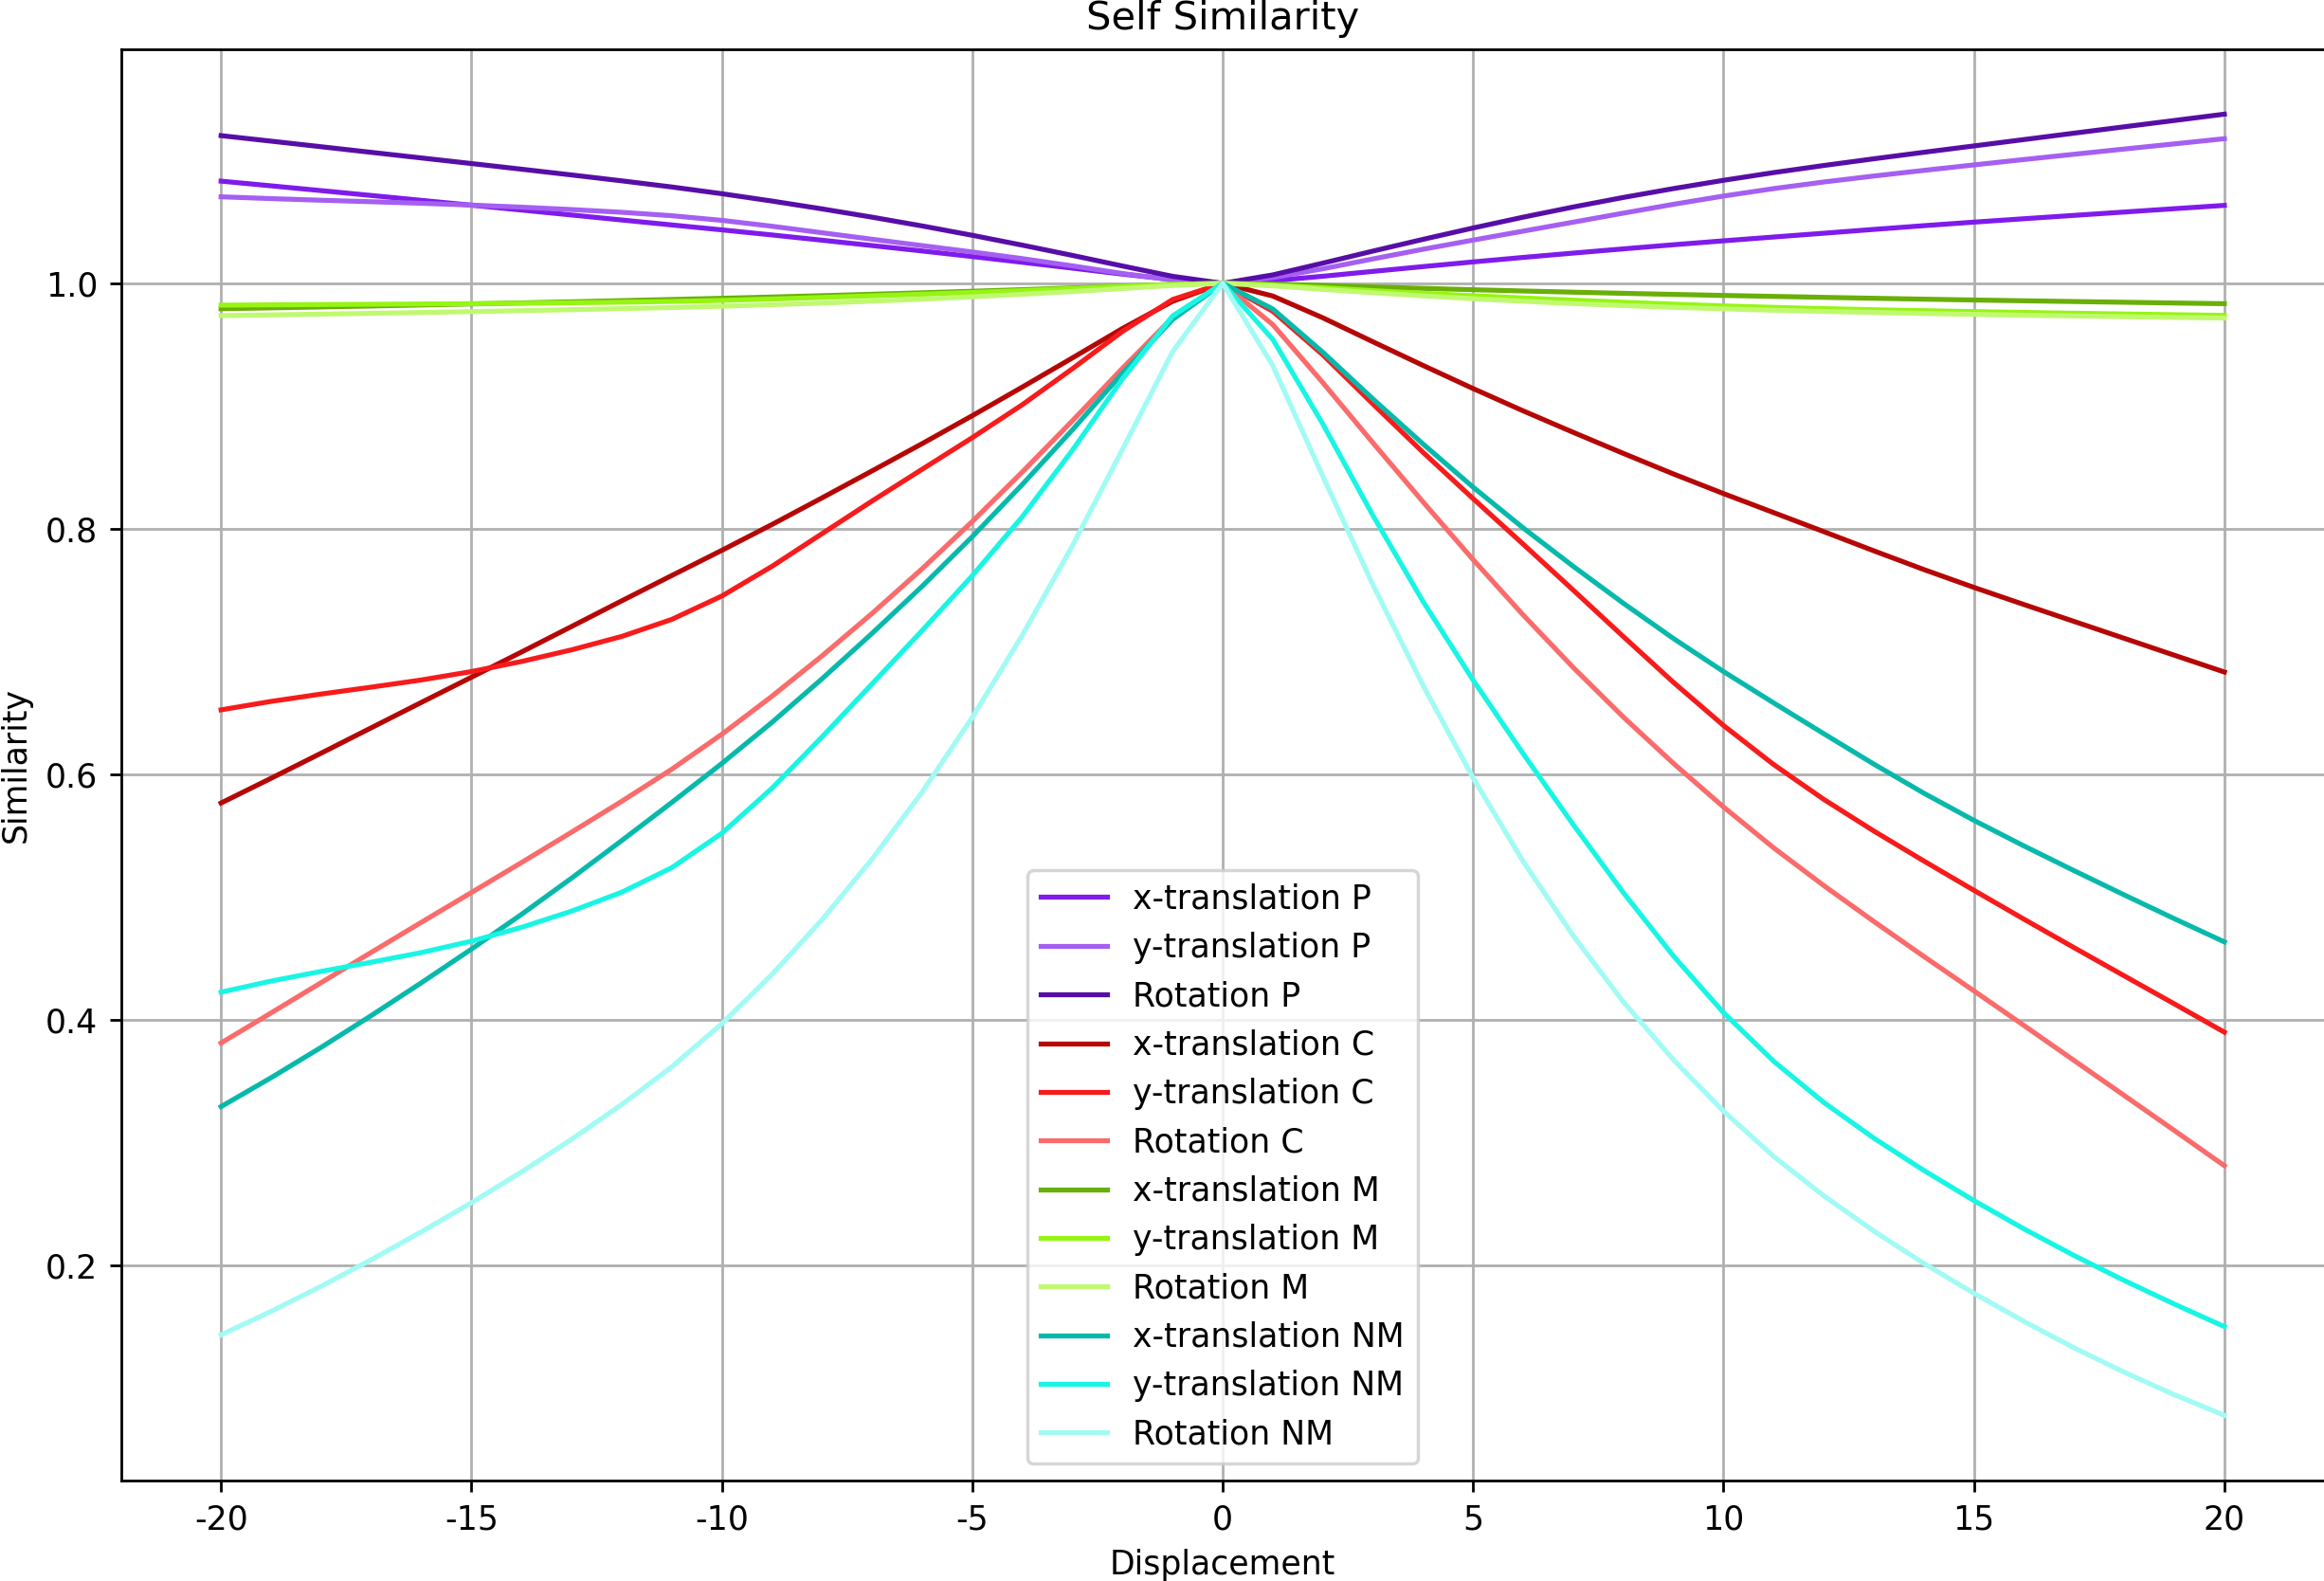
\includegraphics[width=0.8\linewidth]{Materials/selfSimilarity}
	\caption{Self similarity results normalized such that all optima touch 1.0. Both images have been blurred by a Gaussian kernel with sigma being 1. Translation displacement is measured in pixels and rotation displacement is measured in degrees. P = P-norm with P being 2, C = normalized cross correlation, M = mutual information, NM = normalized mutual information.}
	\label{self}
\end{figure}
From the results we note that all similarity measures should be maximized with the exception of P-norm, and thus the P-norm goes above 1.0. We can also see that the similarity measure with the biggest relative difference is NMI, which means NMI both have the greatest gradients, but also is the most sensitive to displacements. In comparison, we see that MI is almost completely flat. However, because MI is so flat, it makes the curves more smooth when we get close to 1.0, whereas for NMI we get some uneven sudden changes as we approach 1.0. For all similarity measures we see them 'peak' at 1.0 as expected as the images should be most similar when not displaced. 